\documentclass{EE-dyplom}

% Pakiety dodatkowe (niezawarte w klasie EE-dyplom)
\usepackage[unicode]{hyperref}
\usepackage{amsmath}
\usepackage{titlesec}
\usepackage{enumitem}
\usepackage{float}

% Ręczne definicje polskich nazw (zamiast pakietu babel)
\renewcommand{\abstractname}{Streszczenie}
\renewcommand{\contentsname}{Spis treści}
\renewcommand{\figurename}{Rysunek}
\renewcommand{\tablename}{Tabela}
\renewcommand{\appendixname}{Dodatek}
\renewcommand{\listfigurename}{Spis rysunków}
\renewcommand{\listtablename}{Spis tabel}
\renewcommand{\refname}{Bibliografia}

% Dane o pracy
\uczelnia{Politechnika Warszawska}
\wydzial{Wydział Mechaniczny Energetyki i Lotnictwa}
\rodzajpracy{PRACA DYPLOMOWA MAGISTERSKA}
\album{321126}
\promotor{dr hab. inż.  Robert Głębocki}

% Dane o pracy (standardowe)
\title{Opracowanie i implementacja niskokosztowego systemu pozycjonowania optycznego dla bezzałogowych statków powietrznych w środowisku zamkniętym}
\author{Paweł Kwiatkowski}
\date{2026}

\begin{document}

\pagenumbering{Alph} % Zapobiega błędom hyperref "destination with the same identifier"
\sloppy
\maketitle

\newpage
\pagenumbering{arabic}
\setcounter{page}{1}

\begin{abstract}
Niniejszy dokument stanowi raport wstępny określający cele, zakres oraz metodykę realizacji pracy dyplomowej dotyczącej budowy systemu nawigacji dla dronów wewnątrz budynków. Głównym celem pracy jest stworzenie niskokosztowego systemu Motion Capture opartego na kamerach konsumenckich (PS3 Eye) oraz aktywnych znacznikach IR, zdolnego do precyzyjnego pozycjonowania UAV w czasie rzeczywistym. Raport przedstawia analizę tła rynkowego, przegląd istniejących rozwiązań (State of the Art) oraz szczegółowy opis planowanej architektury sprzętowej i programowej.
\end{abstract}

\newpage
\tableofcontents
\newpage

\section{Wstęp}

\subsection{Tło rynkowe i motywacja}
W ostatnich latach obserwuje się gwałtowny rozwój rynku bezzałogowych statków powietrznych (UAV). Prognozy rynkowe wskazują na dynamiczny wzrost sektora logistyki dronowej, z przewidywanym średniorocznym tempem wzrostu (CAGR) na poziomie 45.5\% w najbliższej dekadzie. Kluczowym obszarem, który wciąż napotyka bariery technologiczne, jest logistyka tzw. ,,ostatniej mili'' oraz automatyzacja procesów wewnątrz dużych obiektów kubaturowych (magazyny, hale produkcyjne).

W środowiskach tych (tzw. \textit{GPS-denied environments}) standardowe systemy nawigacji satelitarnej są niedostępne lub niewystarczająco precyzyjne. Jednocześnie rośnie zapotrzebowanie na autonomiczne systemy transportowe nie tylko w przemyśle, ale i w zastosowaniach domowych. Poniższy rozdział przedstawia konkretne przykłady wdrożeń dronów wewnątrz budynków, które uzasadniają potrzebę rozwoju niskokosztowych systemów pozycjonowania.

\subsection{Cel i zakres pracy}
Celem głównym pracy jest opracowanie, budowa i weryfikacja eksperymentalna niskokosztowego, zewnętrznego systemu pozycjonowania optycznego (Motion Capture). System ten ma działać w architekturze ,,off-board'', gdzie kamery umieszczone w pomieszczeniu śledzą pozycję drona i przesyłają do niego dane korygujące.

\textbf{Teza pracy:} Możliwe jest osiągnięcie precyzji pozycjonowania wystarczającej do stabilnego zawisu i prostych manewrów wewnątrz pomieszczeń przy użyciu budżetowych sensorów wizyjnych (kamera PS3 Eye) i autorskiego oprogramowania, stanowiąc alternatywę dla kosztownych systemów komercyjnych.

Zakres pracy obejmuje:
\begin{itemize}
    \item Adaptację sprzętową kamer konsumenckich do pracy w podczerwieni.
    \item Budowę aktywnego systemu znaczników IR na platformie latającej.
    \item Implementację algorytmów detekcji i triangulacji pozycji 3D.
    \item Integrację systemu wizyjnego z kontrolerem lotu drona.
\end{itemize}

\section{Zastosowania dronów wewnątrz budynków}

Rozwój systemów pozycjonowania wewnątrzbudynkowego otwiera drogę do szeregu praktycznych zastosowań bezzałogowych statków powietrznych w środowiskach zamkniętych. Poniżej przedstawiono kontekst rynkowy oraz kluczowe obszary aplikacyjne stanowiące motywację dla niniejszej pracy.

\subsection{Kontekst rynkowy}

Rynek logistyki dronowej przeżywa dynamiczny wzrost napędzany rozwojem e-commerce i postępem technologicznym. Według Future Market Insights wartość rynku w 2025 roku wynosi 2,1 mld USD, z prognozą wzrostu do 87,6 mld USD do 2035 roku (CAGR 45,5\%) \cite{fmi2025}. Najbardziej dynamiczny rozwój przewidywany jest po 2030 roku, odzwierciedlając masową adopcję dronów w różnych sektorach przemysłu (Rysunek \ref{fig:market}).

\begin{figure}[H]
    \centering
    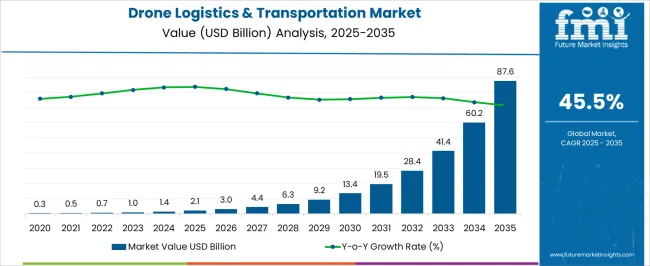
\includegraphics[width=0.9\textwidth]{../../images/Market Context.png}
    \caption{Prognoza wartości rynku logistyki dronowej w latach 2020-2035 \cite{fmi2025}.}
    \label{fig:market}
\end{figure}

Kluczowymi czynnikami wzrostu są zwiększone inwestycje w infrastrukturę, innowacje technologiczne poprawiające żywotność baterii i autonomiczną nawigację, rozwój ram regulacyjnych oraz rosnąca akceptacja społeczna dla transportu dronowego. Według prognoz do 2025 roku liczba dostaw dronowych może osiągnąć 3 miliony dziennie, a około 27,5\% firm planuje wdrożenie rozwiązań logistycznych opartych na dronach \cite{technavio2024}.

\subsection{Załadunek i dostawa paczek}

Drony w zamkniętych magazynach automatyzują proces przygotowania przesyłek do wysyłki, odbierając paczki z różnych stref kompletacji i transportując je do stanowisk konsolidacyjnych lub bezpośrednio do pojazdów dostawczych \cite{cichosz2020}. Załadunek wewnątrz budynku chroni przesyłki przed warunkami atmosferycznymi (deszcz, śnieg, mróz) i eliminuje potrzebę wielokrotnego przemieszczania towarów między strefami.

System pozwala na osiągnięcie 40 dostaw na godzinę z ładunkiem do 10 funtów (ok. 4,5 kg), przy czym testowana automatyzacja umożliwia jednemu operatorowi nadzorowanie do 20 równoczesnych misji dronów. Automatyczne stacje dokowania pozwalają dronom na ładowanie baterii i odbieranie kolejnych przesyłek bez interwencji człowieka, co potencjalnie rozszerza zasięg operacyjny na cały kompleks logistyczny.

Wizja przyszłości zakłada magazyny, w których drony transportują pudła między strefami i wykonują paletyzację bez potrzeby stałych paletyzatorów. Trasy kompletacji mogą być rekonfigurowane poprzez zmianę programowania dronów, a palety budowane tam gdzie są potrzebne, co znacząco poprawia wykorzystanie przestrzeni magazynowej \cite{logisticsbureau2024}.

\subsection{Inwentaryzacja i inspekcja magazynów}

Drony autonomiczne przeprowadzają audyty zapasów w czasie rzeczywistym, skanując tysiące lokalizacji magazynowych w ułamku czasu wymaganego przez zespoły ludzkie. Inwentaryzacje, które tradycyjnie zajmowały dni lub całe weekendy z wyłączeniem operacji, mogą być teraz wykonywane w ciągu godzin bez przerywania normalnej pracy magazynu \cite{aeologic2025}.

IKEA wdrożyła ponad 250 dronów w 73 lokalizacjach w 9 krajach, które pracują 24/7 obok pracowników, przeprowadzając równoczesne kontrole zapasów bez blokowania alejek i zakłócania przepływu pracy \cite{talkinglogistics2024}. System eliminuje fizycznie wyczerpujące zadanie wspinania się na wysokie poziomy regałów (poziom 3 i wyżej), co radykalnie poprawia bezpieczeństwo pracowników i pozwala im skupić się na lżejszych i bardziej wartościowych zadaniach.

Drony wykrywają także anomalie jak zablokowane alejki, zgubione palety, uszkodzone opakowania i puste miejsca, generując automatyczne alerty zanim problemy wpłyną na operacje. Studium przypadku Jaguar Land Rover pokazuje zastosowanie dronów do autonomicznych inspekcji terminali i hal produkcyjnych, gdzie rozwiązanie pozwoliło zaoszczędzić średnio 15 minut podczas załadunku i rozładunku przyczep \cite{autologistics2025}.

\subsection{Transport robotów sprzątających}

Drony stanowią mobilną platformę transportową dla robotów sprzątających, rozwiązując fundamentalny problem urządzeń naziemnych - niemożność pokonywania schodów i przemieszczania się między piętrami budynków. Na targach CES 2026 firma Dreame (subbrand MOVA) zaprezentowała Pilot 70 - system, w którym dron autonomicznie lokalizuje robota odkurzającego, podnosi go za pomocą specjalnego mechanizmu chwytającego, przenosi na żądane piętro lub balkon, a następnie wraca po niego po zakończeniu czyszczenia \cite{cnet2026}.

Koncepcja eliminuje potrzebę posiadania osobnych robotów dla każdego piętra domu, radykalnie zmieniając ekonomię automatyzacji sprzątania w budynkach wielopoziomowych. System HELIOS stosuje podobne podejście do automatycznego czyszczenia paneli solarnych - dron umieszcza małe roboty czyszczące na instalacji fotowoltaicznej, a po zakończeniu pracy odbiera je z powrotem, realizując całą usługę bez obecności właściciela \cite{artrobotics2025}.

\subsection{Podsumowanie zastosowań}

Przedstawione przykłady wdrożeń pokazują, że zapotrzebowanie na precyzyjne systemy pozycjonowania wewnątrzbudynkowego jest realne i rosnące. Wszystkie opisane aplikacje wymagają stabilnego zawisu, precyzyjnego dokowania oraz autonomicznej nawigacji w ograniczonej przestrzeni - funkcjonalności, które są trudne do osiągnięcia dla budżetowych konstrukcji bez zewnętrznego wsparcia nawigacyjnego. Stanowi to bezpośrednią motywację dla niniejszej pracy.

\section{Przegląd literatury i dostępnych rozwiązań}

Nawigacja wewnątrz budynków stanowi wyzwanie badawcze, do którego podchodzi się na wiele sposobów. Poniżej przedstawiono przegląd głównych technologii pozycjonowania stosowanych w środowiskach GPS-denied, wraz z ich charakterystyką, zaletami i ograniczeniami.

\subsection{Markery ArUco}

Markery ArUco stanowią wizyjną metodę nawigacji opartą na sztucznych markerach fiducjalnych, które mogą być wykrywane przez kamerę zamontowaną na dronie. System wykorzystuje czarno-białe wzory binarne w formie kwadratowych markerów, które można wydrukować na zwykłym papierze, co czyni technologię niezwykle tanią i łatwą do skalowania \cite{aruco2025}. Kamera drona wykrywa markery w obrazie, a algorytm estymacji pozy (PnP - Perspective-n-Point) oblicza sześciostopniową pozę kamery względem markera.

Dokładność pozycjonowania zależy od liczby widocznych markerów - z 5 lub większą liczbą markerów błędy są znacznie niższe niż przy mniejszej liczbie. Badania pokazują, że markery ArUco zapewniają najlepszą dokładność w zakresie 0,25-2 metry, przy czym dokładność spada wraz ze wzrostem odległości \cite{aruco_its2025}. Kluczowym ograniczeniem jest zasięg detekcji - optymalna detekcja następuje do około 2 metrów. ArUco jest często stosowany w połączeniu z czujnikami inercyjnymi (IMU) oraz filtrami Kalmana, aby zapewnić ciągłość nawigacji w przypadku utraty kontaktu wzrokowego z markerami.

\begin{figure}[H]
    \centering
    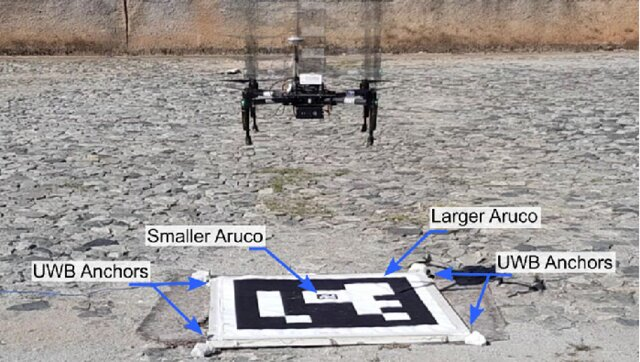
\includegraphics[width=0.5\textwidth]{../../images/Aruco Markers.jpg}
    \caption{Dron z systemem pozycjonowania opartym na markerach ArUco }
    \label{fig:aruco}
\end{figure}

\subsection{Ultradźwięki}

Systemy pozycjonowania ultradźwiękowego wykorzystują sygnały akustyczne o wysokiej częstotliwości emitowane przez stacjonarne nadajniki (beacons), które są odbierane przez mikrofony zamontowane na dronie. Technologia opiera się na pomiarach czasu przelotu sygnału (Time-of-Flight) oraz multilateracji, gdzie pozycja drona jest obliczana na podstawie różnic w czasie docierania sygnałów z co najmniej trzech nadajników \cite{ultrasound_pmc2018}.

Systemy ultradźwiękowe osiągają dokładność pozycjonowania na poziomie centymetrowym - komercyjne rozwiązania jak Marvelmind mogą zapewnić precyzję około 2 cm, podczas gdy typowe implementacje osiągają 9-10 cm dokładności. Systemy hybrydowe łączące ultradźwięki z kamerami Time-of-Flight mogą zapewnić dokładne pozycjonowanie 3D \cite{geoscan2018}. Kluczową zaletą sygnałów akustycznych jest brak penetracji przez ściany, co eliminuje wielodrożność charakterystyczną dla systemów radiowych. Główne ograniczenia to wrażliwość na warunki środowiskowe - turbulencje powietrza, temperatura, wilgotność oraz hałas wpływają na dokładność pomiarów.

\begin{figure}[H]
    \centering
    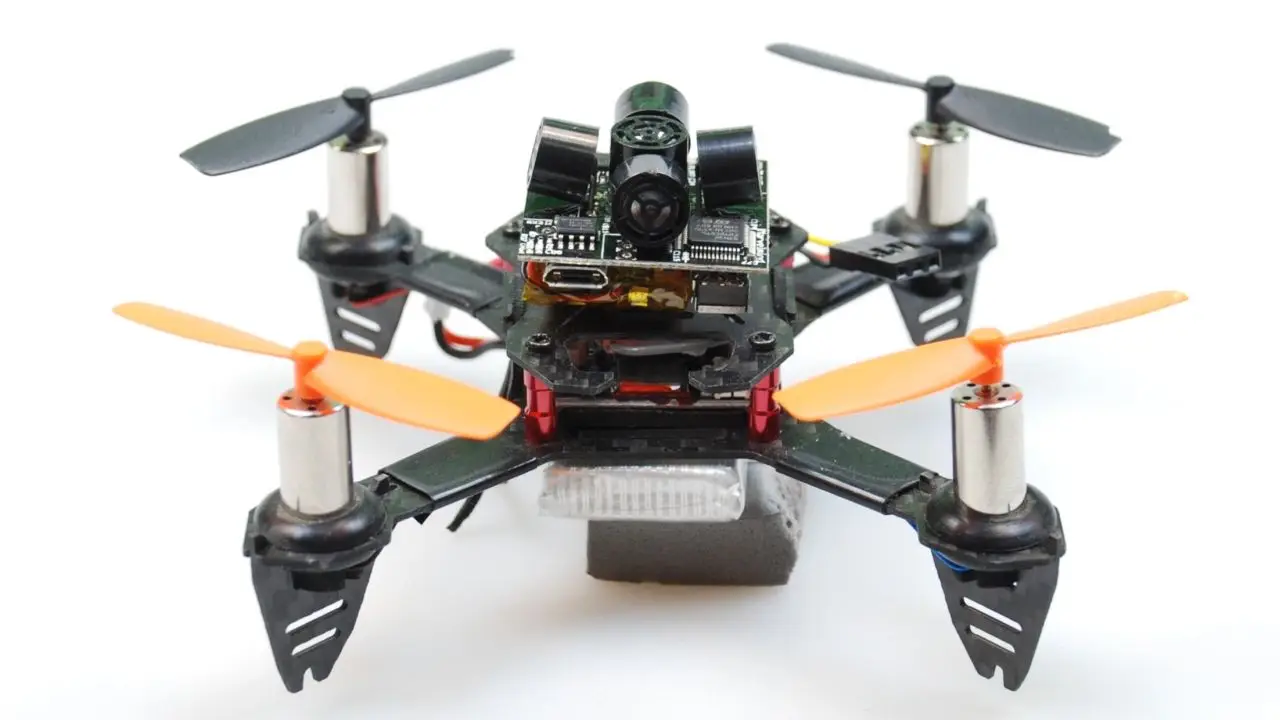
\includegraphics[width=0.5\textwidth]{../../images/Ultrasound.png}
    \caption{Dron z systemem pozycjonowania ultradźwiękowego.}
    \label{fig:ultrasound}
\end{figure}

\subsection{LiDAR / SLAM}

Technologia LiDAR w połączeniu z algorytmami SLAM (Simultaneous Localization and Mapping) stanowi jedno z najbardziej precyzyjnych rozwiązań dla nawigacji wewnętrznej dronów. System LiDAR emituje impulsy laserowe i mierzy czas ich powrotu, generując chmury punktów o wysokiej rozdzielczości \cite{lidar_irjweb}. Algorytmy SLAM przetwarzają te dane w czasie rzeczywistym, umożliwiając jednoczesną lokalizację i budowanie mapy środowiska.

Systemy te osiągają precyzję na poziomie centymetrowym - komercyjne rozwiązania jak Elios 3 z systemem Flyaware zapewniają dokładność 6 cm w trybie czasu rzeczywistym i 2 cm po przetworzeniu \cite{mfe_elios2024}. Kluczowym wyzwaniem w środowiskach dynamicznych jest oddzielenie elementów statycznych od ruchomych. Główne wady technologii LiDAR to wysoka masa sensorów, znaczny koszt sprzętu oraz duże zapotrzebowanie na moc obliczeniową - system musi przetwarzać gęste chmury punktów w czasie rzeczywistym.

\begin{figure}[H]
    \centering
    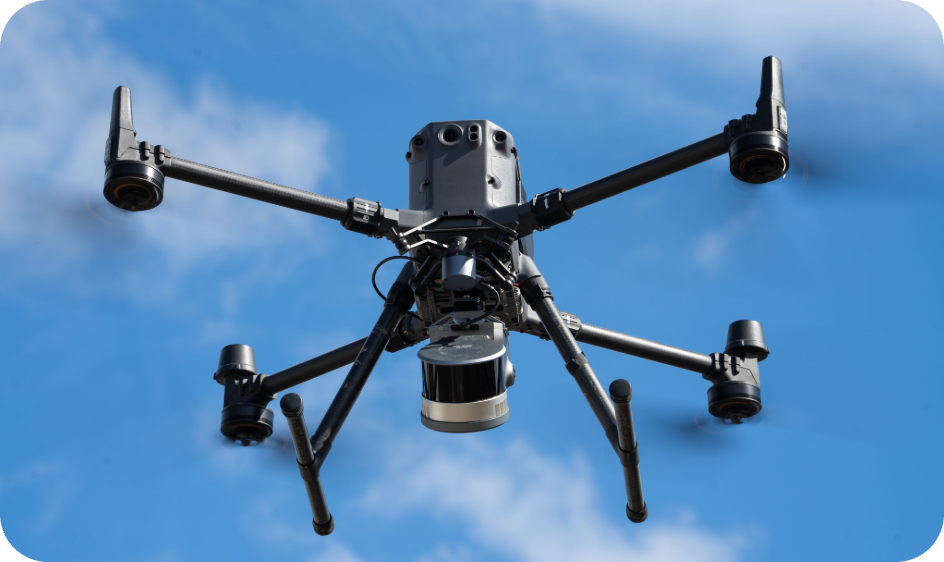
\includegraphics[width=0.5\textwidth]{../../images/Lidar.png}
    \caption{Dron wyposażony w skaner LiDAR do nawigacji SLAM.}
    \label{fig:lidar}
\end{figure}

\subsection{Wizyjna Odometria Inercyjna (VIO)}

VIO stanowi popularne rozwiązanie typu ,,on-board'', łączące dane z kamer z pomiarami IMU w celu precyzyjnej estymacji pozycji drona. System wykrywa i śledzi cechy wizualne (feature points) na kolejnych klatkach obrazu, jednocześnie fuzując te informacje z pomiarami inercyjnymi \cite{vio_pmc2024}. Nowoczesne implementacje osiągają latencję 5-10 ms, demonstrując możliwość pracy w czasie rzeczywistym nawet na platformach o ograniczonych zasobach.

Metoda VIO jest szeroko stosowana w komercyjnych produktach (np. DJI) ze względu na relatywnie niski koszt i małą masę sensorów. Głównym problemem tej technologii jest zawodność w trudnych warunkach oświetleniowych oraz w środowiskach o ubogiej lub jednolitej teksturze. Badania pokazują, że mimo doskonałych wyników na datasetach, algorytmy VIO często zawodzą w realnych warunkach ze względu na zakłócenia zewnętrzne i niestabilne oświetlenie \cite{vio_arxiv2023}.


\subsection{Technologia radiowa UWB}

UWB (Ultra Wide Band) to technologia pozycjonowania wewnętrznego oparta na krótkich impulsach radiowych o wysokiej częstotliwości, która osiągnęła dużą popularność w zastosowaniach przemysłowych. System wykorzystuje pomiary czasu przelotu sygnału (Time-of-Flight) lub różnic czasu przybycia (TDoA) między tagiem na dronie a stacjami bazowymi \cite{uwb_elsevier2023}.

Typowa dokładność pozycjonowania UWB wynosi 10-30 cm, przy czym w przestrzeni 2D można osiągnąć 10 cm, natomiast w 3D dokładność spada do około 30 cm. System oferuje częstotliwość odświeżania do 200 Hz przy opóźnieniu zaledwie 5 ms. UWB charakteryzuje się wysoką odpornością na wielodrożność oraz niskim opóźnieniem, co czyni go idealnym dla złożonych środowisk jak fabryki czy magazyny \cite{uwb_tmk2025}. Główne ograniczenia to niedostateczna precyzja dla aplikacji wymagających dokowania z dokładnością centymetrową.

\subsection{Systemy Motion Capture (MoCap)}

Systemy Motion Capture stanowią jedno z najbardziej precyzyjnych rozwiązań do pozycjonowania dronów w środowiskach GPS-denied, wykorzystywane głównie w laboratoriach badawczych. Technologia opiera się na sieci kamer podczerwieni, które wykrywają refleksyjne markery umieszczone na dronie \cite{px4_mocap2025}. Najpopularniejsze systemy komercyjne to VICON, OptiTrack, NOKOV i Qualisys, które osiągają dokładność pozycjonowania na poziomie submilimetrowym - system VICON Tracker 4 oferuje precyzję do 0,017 mm \cite{vicon2025}.

Systemy te zapewniają tracking w czasie rzeczywistym z niskim opóźnieniem, dostarczając kompletne dane o sześciu stopniach swobody (6DoF). Motion capture umożliwia estymację stanu pojazdu, służy jako ground-truth w eksperymentach lokalizacyjnych oraz wspiera szybkie prototypowanie systemów autonomicznych. Główne ograniczenia technologii to bardzo wysoki koszt infrastruktury, konieczność instalacji wielu kamer oraz ograniczony zasięg działania do przygotowanego wcześniej pomieszczenia. Z tych powodów systemy MoCap są wykorzystywane niemal wyłącznie w ośrodkach akademickich i centrach R\&D.

\begin{figure}[H]
    \centering
    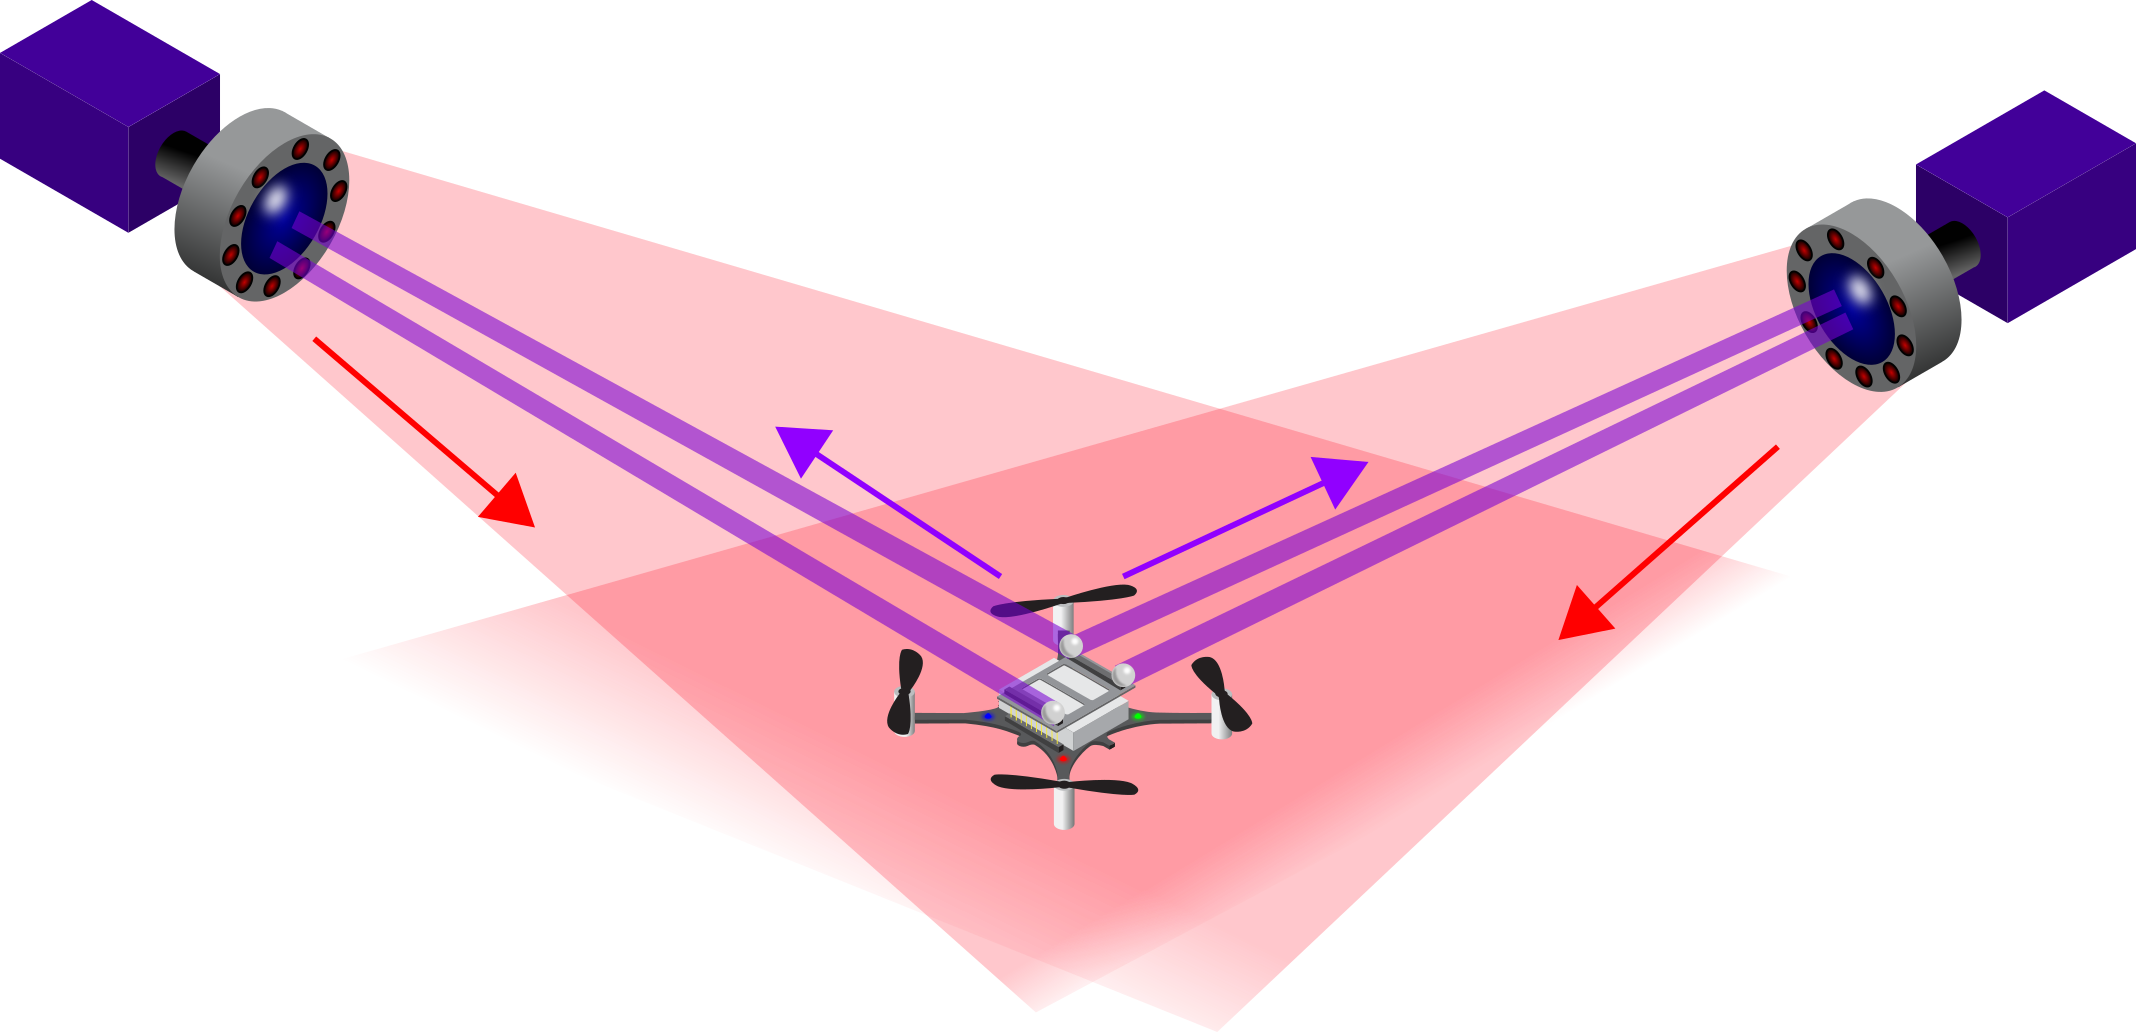
\includegraphics[width=0.55\textwidth]{../../images/Optical Infrared Motion Capture.png}
    \caption{Zasada działania systemu Motion Capture }
    \label{fig:mocap}
\end{figure}

\section{Uzasadnienie wyboru technologii}

\subsection{Analiza porównawcza metod pozycjonowania}

Na podstawie przeglądu literatury przeprowadzono analizę porównawczą dostępnych technologii pod kątem kluczowych wymagań dla nawigacji dronów wewnątrz budynków: precyzji, opóźnienia, kosztu oraz złożoności wdrożenia.

\begin{itemize}
    \item \textbf{Markery ArUco} - bardzo tanie i łatwe w instalacji, jednak ograniczony zasięg detekcji (do 2 m) oraz konieczność montażu kamery na dronie zwiększają masę i pobór energii platformy latającej.
    \item \textbf{Ultradźwięki} - dokładność centymetrowa przy niskim koszcie, lecz wrażliwość na turbulencje powietrza generowane przez wirniki drona oraz ograniczenia środowiskowe (temperatura, wilgotność) wykluczają niezawodne działanie.
    \item \textbf{LiDAR/SLAM} - najwyższa precyzja i autonomia, jednak wysoka masa sensorów, koszt rzędu tysięcy dolarów oraz zapotrzebowanie na moc obliczeniową czynią tę technologię nieosiągalną dla budżetowych konstrukcji.
    \item \textbf{VIO} - popularne rozwiązanie komercyjne, jednak zawodność w warunkach słabego oświetlenia i jednolitych tekstur (typowych dla magazynów i hal) stanowi krytyczne ograniczenie.
    \item \textbf{UWB} - atrakcyjny stosunek ceny do wydajności, lecz dokładność 10-30 cm jest niewystarczająca dla precyzyjnego dokowania i manewrów w ograniczonej przestrzeni.
    \item \textbf{Motion Capture} - submilimetrowa precyzja i niskie opóźnienie, jednak koszt systemów komercyjnych (VICON, OptiTrack) sięgający dziesiątek tysięcy dolarów wyklucza zastosowania poza laboratoriami badawczymi.
\end{itemize}

Spośród analizowanych metod, technologia Motion Capture oferuje najlepsze parametry pod względem precyzji i opóźnienia 
Główną barierą wdrożenia tej technologii jest wysoki koszt infrastruktury. 




\subsection{Koncepcja niskokosztowego systemu MoCap}

W ramach niniejszej pracy postanowiono zweryfikować, czy możliwe jest osiągnięcie użytecznej precyzji pozycjonowania przy zastosowaniu komponentów o koszcie stanowiącym ułamek ceny systemów profesjonalnych. Proponowane podejście opiera się na następujących założeniach:

\begin{enumerate}
    \item \textbf{Tanie kamery konsumenckie} - zamiast specjalistycznych kamer IR o wysokiej czułości, wykorzystanie zmodyfikowanych kamer Sony PS3 Eye (koszt jednostkowy: ok. 20-30 zł na rynku wtórnym), które po usunięciu filtra IR-cut mogą rejestrować światło podczerwone.
    
    \item \textbf{Aktywne znaczniki IR} - zamiast pasywnych markerów retrorefleksyjnych wymagających drogich oświetlaczy, zastosowanie diod LED emitujących światło w paśmie bliskiej podczerwieni. Aktywne źródło światła zapewnia wysoki kontrast względem tła nawet przy użyciu tanich matryc CMOS.
    
    \item \textbf{Improwizowane filtry optyczne} - wykorzystanie materiałów o właściwościach blokujących światło widzialne (np. nośnik magnetyczny z dyskietki 3,5''), co eliminuje konieczność zakupu specjalistycznych filtrów pasmowoprzepustowych.
    
    \item \textbf{Architektura off-board} - zastosowanie taniej platformy latającej (dron hobbystyczny) bez zaawansowanego komputera pokładowego wymusza przeniesienie obliczeń wizyjnych na zewnętrzny komputer PC. Takie podejście pozwala wykorzystać pełną moc obliczeniową bez ograniczeń narzucanych przez masę, pobór energii i koszt platformy latającej.
\end{enumerate}

\subsection{Sformułowanie problemu badawczego}

\textbf{Teza pracy:} Możliwe jest zbudowanie niskokosztowego systemu pozycjonowania optycznego typu Motion Capture, zdolnego do precyzyjnego śledzenia drona w czasie rzeczywistym, przy użyciu komponentów konsumenckich o łącznym koszcie nieprzekraczającym 500 zł.

\textbf{Pytania badawcze:}
\begin{enumerate}
    \item Jaką dokładność pozycjonowania można osiągnąć przy użyciu zmodyfikowanych kamer PS3 Eye i aktywnych znaczników IR?
    \item Czy opóźnienie w torze pomiarowym będzie wystarczająco niskie dla stabilnej kontroli lotu w pętli sprzężenia zwrotnego?
    \item Jakie są ograniczenia zasięgu i warunków oświetleniowych dla proponowanego rozwiązania?
\end{enumerate}

\textbf{Główne wyzwania techniczne:}
\begin{itemize}
    \item Osiągnięcie niskich opóźnień (latency $<$ 50 ms) w całym torze: akwizycja - przetwarzanie - transmisja - sterowanie.
    \item Skuteczna filtracja pasma widzialnego przy użyciu materiałów improwizowanych.
    \item Jednoznaczne wyznaczanie orientacji drona przy ograniczonej liczbie znaczników (rozwiązanie problemu \textit{pose ambiguity}).
\end{itemize}

\section{Realizacja systemu}

W ramach pracy zbudowano funkcjonalny prototyp systemu pozycjonowania, składający się z platformy latającej wyposażonej w aktywne znaczniki IR, zmodyfikowanych kamer PS3 Eye oraz systemu komunikacji bezprzewodowej opartej na modułach ESP32.

\subsection{Platforma latająca}

Jako platformę testową wykorzystano lekkiego drona ze śmigłami 55 mm oraz silnikami szczotkowymi w konfiguracji quadrocopter, wyposażonego w kontroler lotu (FC) z oprogramowaniem Betaflight. Na końcach ramion drona zamontowano trzy diody LED emitujące światło w paśmie bliskiej podczerwieni, co zapewni wysoki kontrast względem tła nawet w zmiennych warunkach oświetleniowych.

Układ diod tworzy trójkąt prostokątny równoramienny, co pozwala na jednoznaczne określenie orientacji drona. Diody IR są zasilane napięciem 5V z kontrolera lotu (FC), z zastosowaniem rezystora 150 $\Omega$ dla każdej diody.

\begin{figure}[H]
    \centering
    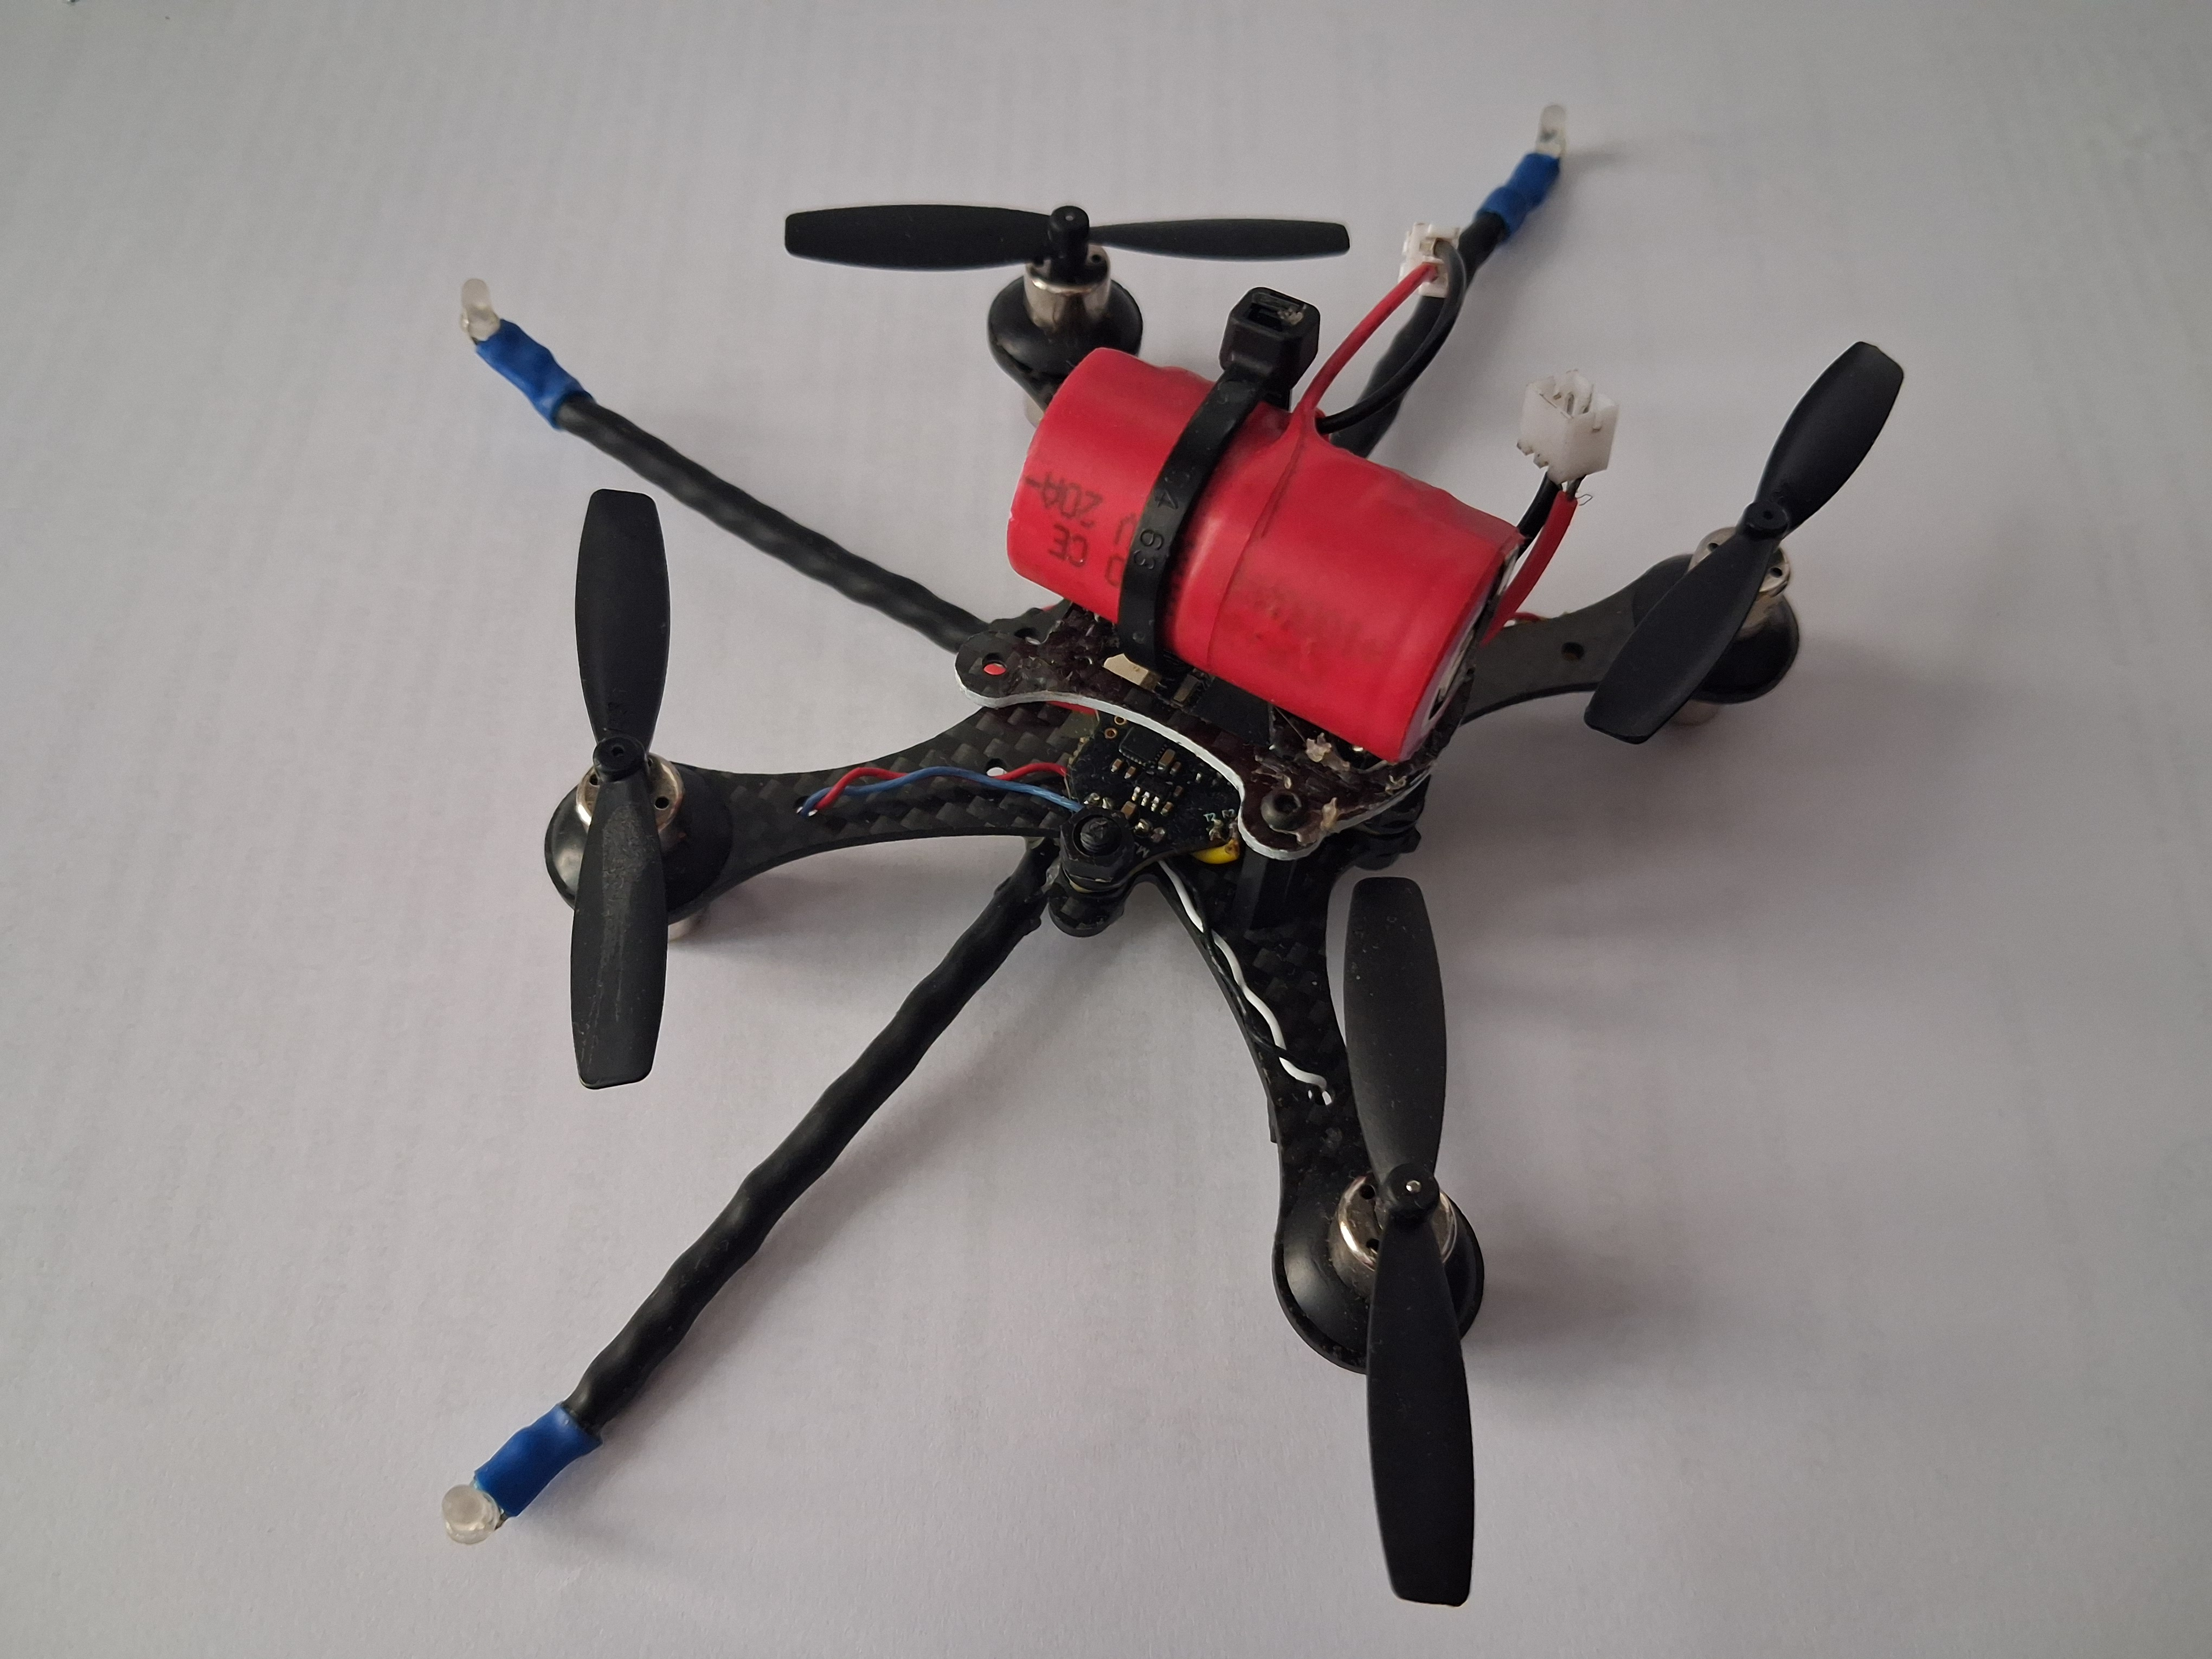
\includegraphics[width=0.7\textwidth]{../../images/drone.jpg}
    \caption{Zbudowany dron testowy z aktywnymi znacznikami IR na końcach ramion.}
    \label{fig:drone}
\end{figure}

\subsection{Modyfikacja kamer PS3 Eye}

Kamery Sony PS3 Eye zostały poddane modyfikacji umożliwiającej pracę w paśmie bliskiej podczerwieni. Proces modyfikacji obejmował trzy etapy:

\begin{enumerate}
    \item \textbf{Usunięcie filtra IR-cut} - fabryczny filtr blokujący podczerwień został zdemontowany z układu optycznego kamery. Filtr ten normalnie chroni matrycę CMOS przed promieniowaniem IR, które mogłoby zaburzać odwzorowanie kolorów.
    
    \item \textbf{Montaż filtra światła widzialnego} - w miejsce usuniętego filtra zamontowano materiał z nośnika magnetycznego (dyskietka 3,5''), który blokuje światło widzialne (poniżej ok. 700 nm), przepuszczając jednocześnie promieniowanie bliskiej podczerwieni. Dzięki temu kamera ,,widzi'' tylko diody IR, ignorując oświetlenie otoczenia.
    
    \item \textbf{Korekcja ogniskowej} - po usunięciu oryginalnego filtra IR-cut zmienia się droga optyczna w kamerze, co powoduje rozogniskowanie obrazu. Problem ten rozwiązano przez przeszlifowanie elementu mocującego obiektyw, co pozwoliło przesunąć soczewkę bliżej matrycy CMOS i przywrócić ostrość obrazu.
\end{enumerate}

Przykładowy obraz z kamery po modyfikacji przedstawiono na Rysunku \ref{fig:camera_view} - widoczne są jedynie trzy jasne punkty odpowiadające diodom IR na dronie, podczas gdy reszta sceny (oświetlenie pomieszczenia, tło) jest całkowicie wyeliminowana przez filtr.

\begin{figure}[H]
    \centering
    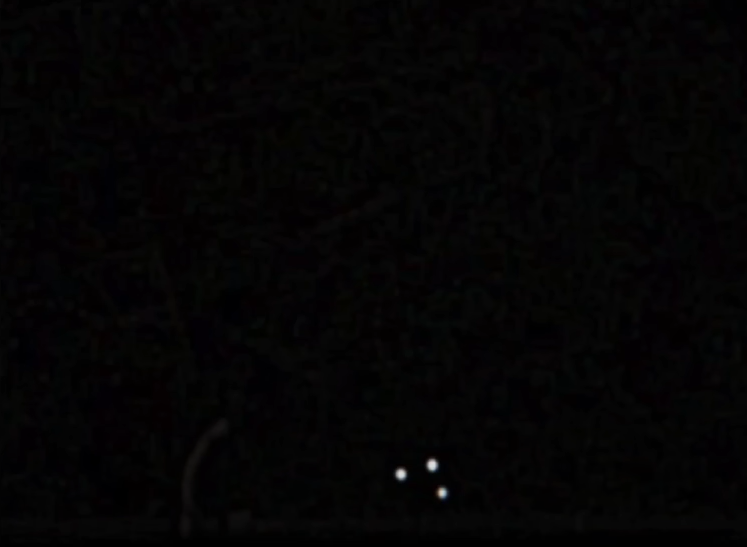
\includegraphics[width=0.6\textwidth]{../../images/image_camera.png}
    \caption{Obraz z zmodyfikowanej kamery PS3 Eye}
    \label{fig:camera_view}
\end{figure}


\subsection{Architektura systemu}

System działa w architekturze off-board, gdzie wszystkie obliczenia wizyjne wykonywane są na zewnętrznym komputerze PC, a do drona przesyłane są jedynie przetworzone dane pozycyjne. Schemat połączeń przedstawiono na Rysunku \ref{fig:schemat}.

\begin{figure}[H]
    \centering
    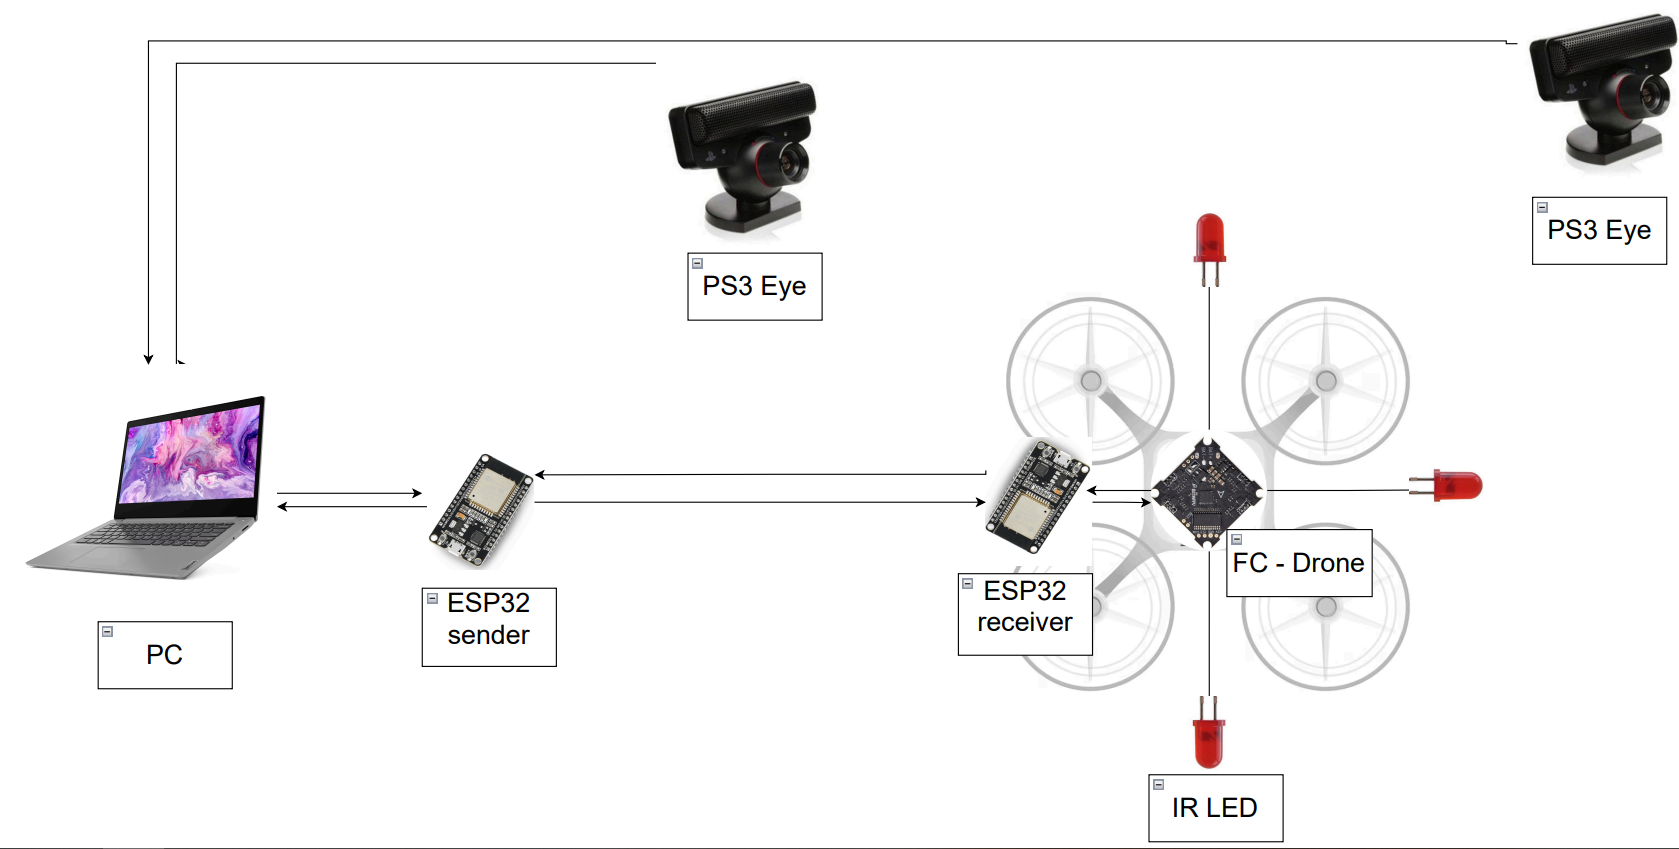
\includegraphics[width=0.95\textwidth]{../../images/schemat.png}
    \caption{Schemat architektury systemu pozycjonowania.}
    \label{fig:schemat}
\end{figure}


Segment naziemny

\begin{itemize}
    \item \textbf{Kamery PS3 Eye} -- podłączone do PC przez USB
    \item \textbf{Komputer PC} -- przetwarza dane z kamer
    \item \textbf{ESP32 sender} -- moduł podłączony do PC przez port szeregowy (USB), odpowiedzialny za transmisję danych pozycyjnych z PC do drona.
\end{itemize}


Segment powietrzny

\begin{itemize}
\item \textbf{ESP32 receiver} - moduł zamontowany na dronie, odbierający bezprzewodowo 
    dane pozycyjne z segmentu naziemnego. Komunikacja między modułami ESP32 realizowana jest z wykorzystaniem 
    protokołu ESP-NOW, zapewniającego możliwe niskie opóźnienia. 
    
    \item \textbf{Kontroler lotu (FC)} - 
    kontroler odpowiedzialny za
    sterowanie silnikami. Komunikuje się z ESP32 receiver przez interfejs szeregowy z 
    wykorzystaniem protokołu MSP (MultiWii Serial Protocol)
    
    \item \textbf{Znaczniki IR LED} - trzy diody podczerwieni zamontowane na ramionach drona, tworzące asymetryczny wzorzec geometryczny.


\section{Harmonogram i oczekiwane wyniki}


\begin{description}[style=nextline]
    \item[Etap 1: Przygotowanie i kalibracja stanowiska pomiarowego (Zrealizowano).] 
    Zmontowano drona testowego wyposażonego w aktywne znaczniki. 
    Przygotowano stanowisko z kamerami PS3 Eye oraz przeprowadzono wstępne testy filtrów optycznych. 
    System komunikacji ESP32 pozwala na transmisję danych pozycyjnych z PC do drona.
    
    \item[Etap 2: Implementacja algorytmów rozpoznawania pozycji.] 
    Opracowanie oprogramowania realizującego:
    \begin{itemize}
        \item Kalibrację wewnętrzną i zewnętrzną kamer.
        \item Segmentację obrazu (progowanie) w celu wykrycia diod.
        \item Dopasowanie wykrytych punktów 2D do modelu geometrycznego trójkąta 
        (rozwiązanie problemu PnP - \textit{Perspective-n-Point} lub triangulacja wielokamerowa).
    \end{itemize}
    
    \item[Etap 3: Implementacja sterowania i kontroli autonomicznej.]
    Zamknięcie pętli sprzężenia zwrotnego.
    Implementacja regulatorów PID odpowiedzialnych za utrzymanie zadanej pozycji (x, y, z) 
    oraz orientacji (yaw). Strojenie parametrów regulatora w celu minimalizacji oscylacji.
    
    \item[Etap 4: Testy w locie.]
    Przeprowadzenie serii eksperymentów weryfikujących:
    \begin{itemize}
        \item Stabilność zawisu (Hover).
        \item Śledzenie prostej trajektorii.
        \item Próbę autonomicznego dokowania (lądowania w wyznaczonym punkcie).
    \end{itemize}
    
    \item[Etap 5:  Analiza danych.]
    Analiza zebranych danych, ocena dokładności systemu oraz sformułowanie wniosków końcowych.
\end{description}


\newpage
\begin{thebibliography}{99}

\bibitem{fmi2025}
Future Market Insights. (2025). Drone Logistics \& Transportation Market - 2035. Dostępne: \url{https://www.futuremarketinsights.com/reports/drone-logistics-transportation-market}

\bibitem{technavio2024}
Technavio. (2024). Drone Logistics And Transportation Market Growth Analysis 2024-2028. Dostępne: \url{https://www.technavio.com/report/drone-transportation-and-logistics-market-industry-analysis}

\bibitem{cichosz2020}
Cichosz, M. (2020). \textit{Drony w logistyce ostatniej mili}. Szkoła Główna Handlowa w Warszawie. Dostępne: \url{https://cor.sgh.waw.pl/bitstream/handle/20.500.12182/959/}

\bibitem{logisticsbureau2024}
Logistics Bureau. (2024). The Future of Drones in Supply Chain Management. Dostępne: \url{https://www.logisticsbureau.com/drones-in-distribution-thinking-inside-the-box/}

\bibitem{autologistics2025}
Automotive Logistics. (2025, 8 grudnia). JLR pilots drone inspections to cut factory downtime and improve safety.

\bibitem{talkinglogistics2024}
Talking Logistics. (2024). Walmart and IKEA: Drone Delivery vs. Drones in the Warehouse. Dostępne: \url{https://talkinglogistics.com/2024/08/26/walmart-and-ikea-drone-delivery-vs-drones-in-the-warehouse/}

\bibitem{aeologic2025}
Aeologic Technologies. (2025). How Drones Are Transforming Warehouse Inventory Management and Tracking. Dostępne: \url{https://www.aeologic.com/blog/how-drones-are-transforming-warehouse-inventory-management-and-tracking/}

\bibitem{cnet2026}
CNET. (2026, 8 stycznia). I Watched a Drone Pick Up a Robot Vacuum and (Sort Of) Carry It Up the Stairs at CES 2026. Dostępne: \url{https://www.cnet.com/home/kitchen-and-household/watched-drone-pick-up-robot-vacuum-carry-it-up-the-stairs-ces-2026/}

\bibitem{artrobotics2025}
ART Robotics. (2025). HELIOS - Automated Cleaning Service for Solar Panels. Dostępne: \url{https://art-robotics.com/cases/helios/}

\bibitem{aruco2025}
arXiv. (2025). Investigation of ArUco Marker Placement for Planar Indoor Localization. Dostępne: \url{https://arxiv.org/html/2509.17345v1}

\bibitem{aruco_its2025}
Institut Teknologi Sepuluh Nopember. (2025). Navigasi Otonom Indoor Drone Menuju Posisi Target Berbasis Pendeteksian Objek dan Penanda ArUco. Dostępne: \url{https://repository.its.ac.id/116380/}

\bibitem{ultrasound_pmc2018}
Paredes, J.A. et al. (2018). 3D Indoor Positioning of UAVs with Spread Spectrum Ultrasound and Time-of-Flight Cameras. PMC/Sensors. Dostępne: \url{https://pmc.ncbi.nlm.nih.gov/articles/PMC5795612/}

\bibitem{geoscan2018}
Geoscan. (2018). Pioneer Indoor navigation system - Ultrasonic local navigation system. Dostępne: \url{https://www.geoscan.ru/en/products/pioneer/locus}

\bibitem{lidar_irjweb}
International Research Journal of Innovations in Engineering and Technology. LiDAR SLAM FOR INDOOR ROBOT NAVIGATION IN DYNAMIC ENVIRONMENT. Dostępne: \url{https://www.irjweb.com/LiDAR\%20SLAM\%20FOR\%20INDOOR\%20ROBOT\%20NAVIGATION\%20IN\%20DYNAMIC\%20ENVIRONMENT.pdf}

\bibitem{mfe_elios2024}
MFE. (2024). Elios 3: The First Indoor LiDAR Mapping Drone. Dostępne: \url{https://mfe-is.com/lios-3-the-first-indoor-lidar-mapping-surveying-drone/}

\bibitem{vio_pmc2024}
PMC/MDPI. (2024). Event-Based Visual/Inertial Odometry for UAV Indoor Navigation. Dostępne: \url{https://pmc.ncbi.nlm.nih.gov/articles/PMC11722967/}

\bibitem{vio_arxiv2023}
Bencak et al. (2023). Deployment of Reliable Visual Inertial Odometry Approaches for Unmanned Aerial Vehicles in Real-world Environment. arXiv. Dostępne: \url{https://arxiv.org/abs/2302.01867}

\bibitem{uwb_elsevier2023}
Lin, H.Y. (2023). GNSS-denied UAV indoor navigation with UWB incorporated visual inertial odometry. Measurement, Elsevier. Dostępne: \url{https://www.sciencedirect.com/science/article/abs/pii/S026322412201452X}

\bibitem{uwb_tmk2025}
The Mobile Knowledge. (2025). White paper: Master Indoor Positioning with UWB Technology. Dostępne: \url{https://www.themobileknowledge.com/knowledge-base/white-paper-master-indoor-positioning-with-uwb-technology/}

\bibitem{px4_mocap2025}
PX4 Documentation. (2025). Flying with Motion Capture (VICON, NOKOV, Optitrack). Dostępne: \url{https://docs.px4.io/main/en/tutorials/motion-capture}

\bibitem{vicon2025}
Vicon Motion Systems. (2025). Motion Capture Systems for Drone Tracking and UAVs. Dostępne: \url{https://www.vicon.com/applications/engineering/autonomous-vehicles/}

\end{thebibliography}

\end{document}